\section{CommunityFinder Software}

\subsection{Overview}
CommunityFinder identifies the community structure in a set of forum posts. It does this by infering the strength of a pair of students' relationship based on how often they make posts to each other. After this structure is determined for all students, CommunityFinder offers two methods of inferring the community structure implied by student interactions. 

\begin{figure}[h]
 \centering
 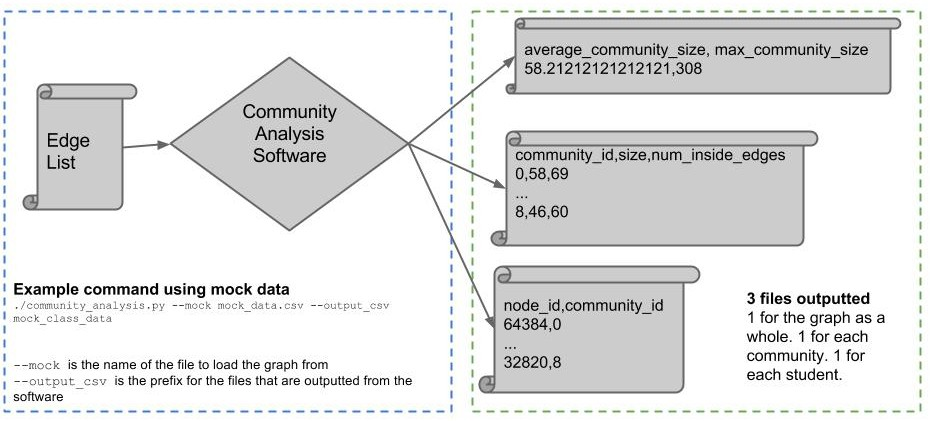
\includegraphics[width=\linewidth]{step2.jpg}
 \caption{CommunityFinder performs analysis on an edge list and output three files that describe the community structure discovered by the graph}
\end{figure}

% \begin{figure}[h]
%  \centering
%  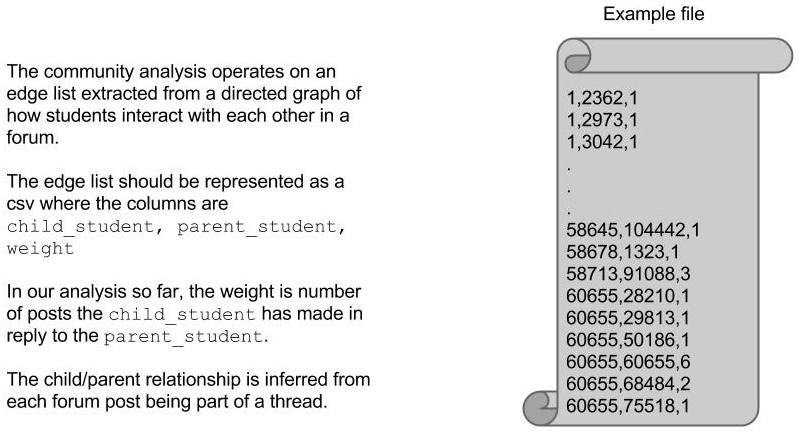
\includegraphics[width=.8\linewidth]{step1.jpg}
%  \caption{The first step in using CommunityFinder is to extract the edge list.}
% \end{figure}


\subsection{Data Sources}
In order to extract an Interaction Graph for analysis, CommunityFinder can query from multiple data sources. Currently, it supports a MySQL database in the MOOCdb \cite{veeramachaneni2013moocdb} format, a Mongo database dump as provied from edX, and an edge list formatted as a file of comma separated values. We recommend using MOOCdb as it is a standardized schema for representing MOOC data.

\subsection{Design Decisions}
CommunityFinder is built with flexibility in mind. It is not meant to be tied to an specific MOOC platform. To this end, it is has support for querying directly from any course data that is in the standardized MOOCDB schema. This is the recommended way to use the software.

\begin{figure}[h]
 \centering
 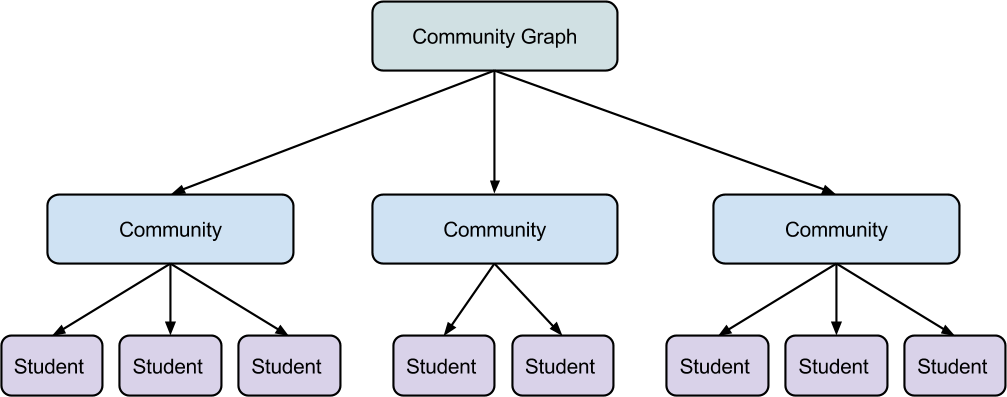
\includegraphics[width=.8\linewidth]{design.png}
 \caption{This represents how the CommnityFinder software understands the structure of the interaction graph. The hierarchical structure was chosen to enable flexibility as the software is developed. }
 \label{design}
\end{figure}

However, it is easy to extend the software to support other data sources. Included in the initial release is support for extracting graph structure from the Mongo database dumps that the edX platform creates. 

Even more, the software supports users who provide their own dataset. An edge list represented as a CSV can be used for analysis by this software. This means that it is possible to use CommunityFinder to find community structure in any graph.

The software organizes the Interaction Graph into a hierarchy of higher level features as shown in Figure \ref{design}. Students are the lowest level. Students are defined by an individual who post on the forum. Student are grouped together to forum communities. A community is a collection of students and has connections to other communities. This hierarchy has a few important implications

\begin{itemize}
\item It is how the data is structured to be exported from the software. This tool is not meant to do analysis beyond community identification. Thus, it is important that the software exports all relevent features about the community structure of the graph that later stages of analysis might use. On the practical side, this structure enabling the programming of additional features for each of the levels. 

\item It gives a good building block for extending functionality. As I discuss the Future Work section, we might want add higher level abstractions such as how the communities develop over time in a class. In order to do this, we simply can create a higher level abstraction that relates several community graph objects.
\end{itemize}

\subsection{Adding Functionality}
Each file that the program outputs is the enumeration of instances of a particular part of the hierarchy in Figure \ref{design}. Right now, these are CommunityGraph, Community, and Student. This means that CommunityFinder outputs a file of comma separated values for each instance at each level. The values that are output depend on the list of properties at the top of each class definition. To add another property, simply add a string to this list. The proprieties can involve additional computation by using python decorators to label certain methods as properties. 
